% !TEX root = ../CINTA-cn.tex
%%%%%%%%%%%%%%%%%%%%%%%%%%%%%%%%%%%%%%%%%%%%%%%%%%%%%%%%%%%%%%%%%%%%
% Author: Libin Wang
% Chapter 6. Group and subgroup
% This document was released as open source on 2026-06-18.
% Copyright 2023, Libin Wang. Creative Commons License
% This work is licensed under a Creative Commons Attribution-NonCommercial-NoDerivatives 4.0 International License.
%%%%%%%%%%%%%%%%%%%%%%%%%%%%%%%%%%%%%%%%%%%%%%%%%%%%%%%%%%%%%%%%%%%

\chapter{群与子群}
\label{chap:group} 

\begin{introduction}
  \item 群
  \item 群的阶
  \item 子群
  \item 群的基本属性
\end{introduction}

\section{群} 
\label{sec:group}
%Motivation. 
前两章的内容主要针对整数的模算术运算，若干定理、引理的推导强烈依赖消去律（命题~\ref{pro:cancel}）。所谓消去律即：
\begin{theorem*}{消去律}{}
对整数$a$，$b$，$c$和$m$，且$\gcd(c, m) = 1$。如果$ac \equiv bc \pmod{m}$，则$a \equiv b \pmod{m}$。
\end{theorem*}

消去律意味着给定互素的整数$a$和$m$，可以计算$a$模$m$的乘法逆元$a^{-1}$，使得$a a^{-1} \equiv 1 \pmod{m}$。
我们利用消去律推导出费尔马小定理~\ref{thm:FLT}和欧拉定理~\ref{thm:euler}。
	
%%Additional conditions.
在这一章的开始，首先需要思考的就是：在前两章的推导过程中，还使用了什么数学属性，但没有明确地定义或指出？
 比如，我们必须使用\emph{结合律}： 

\begin{theorem*}{结合律}{}
对整数$a$，$b$，$c$和$m$，$(ab)c \equiv a(bc) \pmod{m}$。
\end{theorem*}

\begin{thinking} 
请问有什么算术运算或者数学操作不满足结合律？
\end{thinking}
\iffalse
	\begin{center}
	\begin{tcolorbox}[width = 8cm, title = {结合律.}]
	对整数$a$，$b$，$c$和$m$，
	\[(ab)c \equiv a(bc) \pmod{m}\text{。}\]
	\end{tcolorbox}
	\end{center}
\fi	

其次，我们还需要\emph{封闭性}（\emph{closure}）\index{封闭性}\index{closure}。也就是说，借助模运算，比如模整数$m$，我们只需考虑$0$到$m-1$之间的整数。
对于整数和模算术运算，封闭性和结合律显然具备。
%20200521
最后，还需要强调，我们需要整数“$1$”，这是一个重要的且被严重依赖的隐式条件，没有“$1$”，逆元就无从说起了。

%%Wrap up.
综合以上条件，并把它们推广到任意元素的集合$\mathbb{G}$上，就形成一种新的概念：\emph{群}（\emph{group}）\index{group}。
% and an operator $\cdot$  on the elements, we form a new concept named
	
\begin{definition}{群}{grp}
%\label{def:grp}
群是集合 $\mathbb{G}$ 以及在其元素上所定义的操作符$\cdot$，并满足以下公理：
	\begin{itemize}
		\item \emph{封闭性}：$\forall a,b \in \mathbb{G}, \quad a\cdot b \in \mathbb{G}$；
		
		\item \emph{结合律}：$(a\cdot b)\cdot c = a\cdot (b\cdot c)$；
		
		\item 存在一个被称为\emph{单位元}（\emph{identity}）\index{identity}的元素“$e\in \mathbb{G}$”，使得$e\cdot a = a \cdot e = a$；
		
		\item $\forall a\in G$，存在\emph{逆元}（\emph{inverse}）$a^{-1}\in G$，使得$a\cdot a^{-1} = e = a^{-1} \cdot a$。
	\end{itemize}
如果对任意$a, b\in G$，满足$a \cdot b = b \cdot a$，则群$G$被称为阿贝尔群\index{Abelian group}或交换群\index{commutative group} 。
\end{definition}
	
%Examples of groups.
以下给出几种重要的群（或非群）的实例。建议读者自行验证这些实例，明确某些代数结构为什么是或者不是群。
\begin{example}
 $(\mathbb{Z}, +)$ 是群，但$(\mathbb{Z}, \times)$ 不是群。
  $(\mathbb{Q}, +)$ 和 $(\mathbb{R}, +)$ 都是群。同时 $\mathbb{Q}$ 和 $\mathbb{R}$ 抛掉$0$之后在乘法上也形成群。
\end{example}

\begin{example}
 所有的偶数在加法下成群，记为$2\Z$；但是所有奇数加上$0$在加法操作下不是群，因为奇数加奇数可能是偶数，不满足封闭性。
 更一般地，对任意整数$n \in Z$，$n$的所有倍数
 形成的集合$n\Z =\{ kn : k \in \Z\}$在加法上成群。
 直观上，$n$的倍数相加还是$n$的倍数，$0$是单位元，对任意的$a\in \Z$，$na$的逆元是$-na$。
\end{example}
	
\begin{example}%{$\mathbb{Z}_n$}
设$n$为整数，$\mathbb{Z}_n = \{0, 1, 2, \ldots, n-1\}$在模$n$的加法操作下形成群。然而，在模$n$的乘法操作下$(\mathbb{Z}_n, \times)$则不是群。
\end{example}

\begin{example}%{$\mathbb{Z}_p^*$}
设$p$为素数，$\mathbb{Z}_p^* = \{1, 2, \ldots, p-1\}$在模$p$的乘法下形成群。请适时地回忆一下费尔马小定理的证明。
\end{example}

\begin{example}%{$\mathbb{Z}_n^*$}
设$n$为正整数，$\mathbb{Z}_n^* = \{ a \in [1..n-1] \; \text{且} \; \gcd(a,n) =1 \}$在模$n$的乘法下形成群。请回忆欧拉定理。
\end{example}

%20250316 添加
\begin{example}%{$\mathbb{U}_n}
\label{exm:nth_root_of_unity}
	\index{nth root of unity}\index{n次单位根}
	设$n$为正整数，称方程$z^n = 1$在复数上的所有解为$n$次单位根，记为$\mathbb{U}_n = \{ z^n = 1, z \in \mathbb{C}\} $。
	根据高等数学相关知识可知，$\mathbb{U}_n = \{e^{\frac{2\pi i k}{n}}, k = 0, 1, \ldots , n - 1\}$，并且
	\[ e^{\frac{2\pi i k}{n}} = \cos(\frac{2 \pi k}{n}) + i \sin(\frac{2\pi k}{n}), k = 0, 1, \ldots , n - 1\]
	如果记$\omega = \cos(\frac{2 \pi }{n}) + i \sin(\frac{2\pi }{n})$，则可更简洁地表示$n$次单位根为
	\[\mathbb{U}_n = \{\omega^i, i = 0, 1, \ldots , n - 1\}\]
	可证明$\mathbb{U}_n $ 在复数的乘法上形成群(这是课后习题)，并称$\mathbb{U}_n $ 为$n$次单位根群。为直观起见，图~\ref{fig:nth_root_unity}展示了
	$8$次单位根群的群元在单位圆上的位置。
\end{example}

%单位根群
\begin{figure}
	\begin{center}
		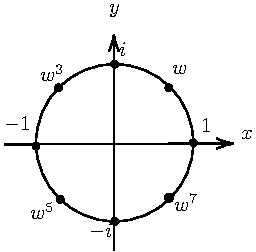
\includegraphics[scale=1.5]{figures/nth-unity.pdf} 	
		\caption{$8$次单位根群}
		\label{fig:nth_root_unity}       % Give a unique label
	\end{center}
\end{figure}

%20250316 添加
\begin{thinking}
	读者能发现$\mathbb{Z}_n$ 与$\mathbb{U}_n$ 的操作行为很类似吗？这会意味什么呢？
	另外，$\mathbb{U}_n$ 的操作行为与$\Z_p^*$不很类似，是吗？%%%我是在挖坑，其实是类似！
\end{thinking}
	
\begin{example}
\label{exm:glg_sl}
实数集合上$n \times n$的可逆矩阵的集合在矩阵乘法下形成群，称为\emph{一般线性群}（\emph{general linear group}），记为$\operatorname{GL}_n(\mathbb{R})$；
\index{一般线性群}\index{general linear group}
实数集合上行列式为$1$的$n \times n$可逆矩阵集合在矩阵乘法下形成群，称为\emph{特殊线性群}（\emph{special linear group}），记为$\operatorname{SL}_n(\mathbb{R})$。
\index{特殊线性群}\index{special linear group}
这两个群都不是阿贝尔群。
\end{example}

\begin{example}
\label{exm:sym_gr}
给定任意一个$n$个元素的集合$S$，存在$n!$个从$S$到$S$的置换，这些置换在函数复合操作下形成群$\mathbb{S}_n$，称之为
\emph{对称群}（symmetric group）\index{对称群}\index{symmetric group}。请读者验证！
\end{example}
 
 %%%20220714 From ST16 第6章
 \begin{example}
 \label{exm:cycle_gr}
设$\mathbb{O}$是所有模为$1$的复数集合，即任取$a + b i \in \mathbb{O}$，则有$\sqrt{a^2 + b^2} = 1$。请读者验证
$\mathbb{O}$在复数乘法上成群。我们称$\mathbb{O}$为\emph{圆圈群}（\emph{cycle group}），
因为本质上，它刻画的是一个半径为$1$的圈圈。我们将在第~\ref{chap:iso_hom}章展示它与群$\mathbb{R}$、$\mathbb{Z}$
之间的关系，一个非常有趣且内涵丰富的结论。
\index{圆圈群}\index{cycle group}
 \end{example}
 
 %20200527
必须强调，就
 严谨性而言，群的定义必须包括两部分，数据集与操作符。然而为了可读性与使用的方便，符号误用无处不在。
 比如，对某些约定俗成的群，加法与乘法含义明确时，我们就不再注明操作符，比如$\Z$、$\Z_p$和$\Z_n$是加法群，
 $\Z_p^*$和$\Z_n^*$是乘法群。再比如，群元素的操作$a \cdot b$往往在不引起误解的时候也写成$ab$。
 为了方便，值得牺牲部分严谨性。
 
\section{群的基本性质} 
\label{sec:prop_gr}
%Basic Properties of Groups.
\begin{proposition}{单位元唯一性}{grp_uniq_1}
群$\mathbb{G}$的单位元唯一；即存在唯一的元素$e \in \mathbb{G}$使得对所有$g\in \mathbb{G}$，有$eg= ge = g$。
\end{proposition}

\begin{proof}
 假设$e, e' \in \mathbb{G}$为单位元，则
 $e e' = e'$，且
 $e e' = e$。联立以上两个等式，得$e = e e' = e'$。\qed
\end{proof}

\begin{proposition}{逆元唯一性}{grp_uniq_2}
		$\forall g \in \mathbb{G}$，$g$ 有唯一逆元$g^{-1}$。
\end{proposition}
	
\begin{proof}
		如果$g^{-1}$和$g'$都是$g$的逆元，则有
		\[ g' = g' e = g' (g g^{-1}) = (g' g)g^{-1} = e g^{-1} = g^{-1}.\]
		 \qed
\end{proof}
	
%20250324 添加
\begin{thinking}
	请回忆，模运算的乘法逆元的唯一性是如何达成的？为什么在一个抽象出来的框架中，逆元的唯一性如此轻易就达成了呢？
	%%%mod运算的乘法逆元需要用到Bezout定理（存在性），然后分析得出唯一性。！
\end{thinking}

\begin{proposition}{}{}
		设$\mathbb{G}$为群，任取$a, b \in \mathbb{G}$，则$(ab)^{-1} = b^{-1} a^{-1}$。
\end{proposition}

	\begin{proof}
		构造法。因为$(ab)(b^{-1}a^{-1}) = e$，且$(b^{-1}a^{-1}) (ab) = e$，所以，根据定义，$ab$的逆元是$b^{-1}a^{-1}$。\qed
	\end{proof}

	\begin{proposition}{}{}
		设$\mathbb{G}$是一个群，对所有群元$ g \in \mathbb{G}$, $(g^{-1})^{-1} = g$。
	\end{proposition}

	\begin{proof}
	根据群公理，$g g^{-1}=e$，且 $g^{-1}(g^{-1})^{-1} = e$。因此：
		\[
		(g^{-1})^{-1} = e(g^{-1})^{-1} =  (g g^{-1}) (g^{-1})^{-1} = g( g^{-1} (g^{-1})^{-1})= ge = g .
		\]
		\qed
	\end{proof}

	\begin{proposition}{}{cong_eq}
	设$\mathbb{G}$为群，任取两个元素$a, b \in \mathbb{G}$，则等式$ax = b$ (或 $xa = b $)在$\mathbb{G}$上有唯一解。
	\end{proposition}
		
	\begin{proof}对于存在性，可找出满足要求的$x$。对唯一性，反证法。假设存在$x_1$和$x_2$都是解，推出矛盾。
	完整证明留作课后练习。\qed
	\end{proof}

	\begin{proposition}{}{cancel_gr}
	%\label{prop:cancel_gr}
	设$\mathbb{G}$为群，且$a, b, c \in \mathbb{G}$。如果$ba = ca$，则$b = c$；并且，如果$ab = ac$，则$b = c$。
	\end{proposition}
	\begin{proof}
		 留作课后练习。\qed
	\end{proof}
命题~\ref{pro:cancel_gr}告诉我们，对于群消去律必然存在。对于非交换群，还分别有左消去律和右消去律。那么，之前依赖消去律
所得的若干属性就立即可以推广到任意的群上去。

\begin{example}
在费尔马小定理和欧拉定理的证明中，依赖消去律我们有：对任意素数$p$和与$p$互素的正整数$a$，
$\Z_p^* =a \Z_p^* = \{ a i : i \in \Z_p^* \}$; 
对任意合数$n$和与$n$互素的正整数$a$，$a \Z_n^* = \Z_n^*$。请问，对任意只有有限个元素的群$\mathbb{G}$和群元$a\in \mathbb{G}$，
是否有$ \mathbb{G} = a \mathbb{G} = \{a g :  g \in \mathbb{G} \} $？为什么？
\end{example}
%A little thought.
%   Where does "\emph{Cancellation Law}" come from?

%%%Permutation Group
%%% 20200617
%%% 20240402
\begin{example}{(置换群)}
\label{exm:perm_gr}
对任意给定的具有$n$个元素的有限群$ \mathbb{G}$，$ \mathbb{G} = a \mathbb{G} = \{a g : g \in \mathbb{G} \} $。
当然，结果并不出人意料。
理解这种性质的一种方法是，把任意群元素$a$“乘”上所有群元素的操作理解为一种映射
$\lambda_a\colon \mathbb{G}  \to \mathbb{G}$，该映射被定义为$\lambda_a(g) = a g$，其中，
$\forall g \in \mathbb{G} $。直观上看，映射$\lambda_a$就是一次\emph{置换}（permutation）操作，它改变了群元素的位置，但群并没有变化。
容易证明，映射$\lambda_a$是一种双射，即同时为单射和满射，证明依然依赖消去律。
对于一个$n$阶有限群$ \mathbb{G}$，天然可以定义出$n$种置换映射，形成一个$n$阶集合：
\[ \overline{\mathbb{G}} = \{ \lambda_g: g \in \mathbb{G} \}\]
有趣的是，在\emph{函数复合}操作下，$\overline{\mathbb{G}} $是一个群。可验证所有群公理，它满足封闭性，因为：
\[ (\lambda_a \circ \lambda_b) (g) = \lambda_a(bg) = abg = \lambda_{ab}(g) \in  \overline{\mathbb{G}} \text{；}\]
有单位元，因为对任意$\lambda_a \in \overline{\mathbb{G}}$：
\[ (\lambda_e \circ \lambda_a)(g) = eag = ag =\lambda_a(g) \text{，}\]
并且
\[ (\lambda_a \circ \lambda_e)(g) = aeg = ag = \lambda_a(g) \text{；}\]
最后，可验证该代数结构有逆元：
\[ (\lambda_a \circ \lambda_{a^{-1}})(g) = \lambda_a(a^{-1}g) = a a^{-1}g = g  = \lambda_e(g) \text{。}\]
这种由若干个置换构成的群被命名为\emph{置换群}（\emph{permutation group}）\index{置换群}\index{permutation group}。
\end{example}

%Notations.
接下来引入一些常用的表达式。设$\mathbb{G}$是群，且$g \in \mathbb{G}$。对任意$n\in \mathbb{N}$，有以下表达式。

    \begin{itemize}
       	\item $g^0 = e$
       	\item $g^n = \underbrace{g\cdot g \cdots g}_{\text{n-1 次群运算}}$
       	\item $g^{-n} = \underbrace{g^{-1}\cdot g^{-1} \cdots g^{-1}}_{\text{n-1 次群运算}}$
    \end{itemize}
    
\begin{remark}
\label{rem:scaler-vs-group-element}
值得强调的是，任意群元$g^i$中的$i$不是群元素，是一个\emph{标量}（\emph{scalar}）。
看上去这种强调没什么意思，其实不然，如果$g$刚好是落在整数上的群，往往会容易混淆。
又偏巧，这种混淆是暂时无害的误解，习惯成自然，到了真要区分标量与群元素的时候往往会忘记了这里的强调。
\end{remark}
另外，如果把群理解为加法群的时候，往往又把$g^i$写成$i g$。比如第~\ref{chap:EC}章的椭圆曲线群，$n$个群元素$P$
自相加就表示为$nP$。

\begin{proposition}{}{grp_expo}
设$\mathbb{G}$是群，$\forall a, b \in \mathbb{G}$，以下性质成立。
\begin{itemize}
\item $\forall m,n \in \Z$，$g^m g^n = g^{m+n}$；

\item $\forall m,n \in \Z$，$(g^m)^n = g^{mn}$；

\item $\forall n \in \Z$，$(gh)^n = (h^{-1}g^{-1})^{-n}$；如果$\mathbb{G}$是阿贝尔群，则$(gh)^n = g^n h^n$。
\end{itemize}
\end{proposition}
\begin{proof}
留做课后练习。\qed
\end{proof}

\begin{definition}{阶}{order}\index{order}
       有限群的\emph{阶}（\emph{order}）被定义为群元素的个数。如果一个群有无穷多元素，则它的阶称为\emph{无穷阶}。
       如果群$\mathbb{G}$有$n$个元素，记为$\vert \mathbb{G} \vert = n$。
       设$g \in \mathbb{G}$，$g$的阶被定义为最小正整数$m$使得$g^m = e$，并记为$\operatorname{ord}(g) = m$。
       如果不存在最小正整数$m$使得$g^m = e$，则称$g$有无穷阶。
 \end{definition}
%20200604
\begin{example}
群$\Z$是无穷阶群。
设$p$是素数，则群$\Z_p$的阶是$p$，群$\Z_p^*$的阶是$p -1$。
设$n$是任意正整数，群$\Z_n$的阶是$n$，群$\Z_n^*$的阶是$\varphi(n)$。
\end{example}

%20200613
\begin{example}
请注意，群元素的阶与群操作相关。比如，加法群$\Z_p$中元素的阶称为加法阶，而乘法群$\Z_p^*$元素的阶则称为乘法阶。
在 Sage 中分别给出了不同的操作。在上下文明确的且无歧义时，常常省略群操作而只称为阶。

\begin{lstlisting}
sage: p = 17; a = 4
sage: Mod(a, p).multiplicative_order()  # a模p的乘法阶，即a在乘法群中的阶
4
sage: Mod(a, p).additive_order()        # a模p的加法阶，即a在加法群中的阶
17
\end{lstlisting}

\end{example}
%20200604
\begin{example}
\label{exm:cyc_gen}
设$p=11$，请编程验证$\Z_p$中除单位元之外的每一个元素阶都为$11$。尝试多个不同的素数，发现规律：
如果$p$是素数，则群$\Z_p$中除单位元之外的每一个元素阶都为$p$。可以验证，$2$在$\Z_{11}^*$中的阶是$10$，
但是并非单位元除外的所有元素的阶都是$10$，比如$4$的阶是$5$。我们会在第~\ref{chap:cyc_grp}章继续讨论这些问题。
\end{example}

\section{子群}
\label{sec:sub_gr}
%20190926
%20200525
要分析一个大的数据集，我们往往会先把数据划分为若干小的集合进行分析。同样地，要考察一个群的属性，
我们也会先把群分成更小的群，先考察小群的属性。
这种想法引出了\emph{子群}（\emph{subgroup}）\index{subgroup}的定义。通过子群来研究群的结构将是以下章节的重要主题。

\begin{definition}{子群}{subg}
    设$\mathbb{G}$为群。若$\mathbb{H}$是$\mathbb{G}$的子集，且$\mathbb{H}$在群$\mathbb{G}$的操作符上也满足群公理，则$\mathbb{H}$
	被称为$\mathbb{G}$的子群，记为$\mathbb{H}\leq \mathbb{G}$。
\end{definition}

	\begin{example}
若干子群的实例。
          \begin{itemize}
            \item 在加法上，偶数群$2\Z$是整数群$\Z$的子群。对任意的$n \in \Z$，$n\Z$是$\Z$的子群。
          
          	 \item 对任意群$\mathbb{G}$，存在一个\emph{平凡子群}$\{ e \}$\index{trivial subgroup}。这是简单且平凡的结论，但值得留意。
          	 
          	 \item 在加法上，$\mathbb{Z} \leq \mathbb{Q} \leq \mathbb{R} \leq \mathbb{C}$。
          	 
          \end{itemize}
	\end{example}
	
\begin{example}{($\Z_p^*$的子群.)}
	\label{exm:zp}
	设$p$为素数，对所有的$i \in \Z_p^*$，计算$i^2 \bmod p$，形成集合$\mathbb{S} = \{ i^2 \bmod p, \forall i \in \Z_p^*\}$。
	检验$\mathbb{S}$在模$p$的乘法下形成群，即$\mathbb{S} \leq \Z_p^*$。$\mathbb{S}$的阶是多少？
\end{example}

\begin{example}{($\Z_n^*$的子群.)} 
	\label{exm:zn}
	设$n$是一个正合数，随机选取两个整数$a, b \in \Z_n^*$，形成集合$\mathbb{S} = \{ a, b\}$。然后，将集合$\mathbb{S}$中两个
	元素相乘得到$c$，如果$c \notin \mathbb{S}$则更新集合$\mathbb{S}$为$\mathbb{S} \cup \{c\}$。不断重复这种操作，
	直到$\mathbb{S}$不再增长。检验$\mathbb{S}$在模$n$乘法操作下形成群，即$\mathbb{S} \leq \Z_n^*$。请计算$\mathbb{S}$的阶。
\end{example}
	
\begin{example}{(对称群的子群就是置换群.)} 
\label{exm:symm_gr}
例子~\ref{exm:sym_gr}中定义了对称群$\mathbb{S}_n$，而例子~\ref{exm:perm_gr}定义了置换群。
一般而言，把对称群的子群定义为置换群。
\end{example}

\begin{example}{(特殊线性群是一般线性群的子群.)} 
\label{exm:gl_subgr}
易知，对于任意整数$n$，特殊线性群$\operatorname{SL}_n(\mathbb{R})$是一般线性群$\operatorname{GL}_n(\mathbb{R})$的子群。
\end{example}

%decide a subgroup.
表面上看，要判定群$\mathbb{G}$ 的非空子集$\mathbb{H}$是否$\mathbb{G}$ 的子群，只需要检查$\mathbb{H}$中的元素是否满足群公理即可。
但是，考虑到群中单位元的唯一性、逆元的唯一性，而且$\mathbb{H}$的元素必然继承了群$\mathbb{G}$的结合律，那么检查条件可以简化，见以下命题。
\begin{proposition}{}{subgr0}
	%\label{prop:subgr}
	群$\mathbb{G}$ 的非空子集$\mathbb{H}$是$\mathbb{G}$ 的子群，当且仅当$\mathbb{H}$同时满足以下条件：
	\begin{itemize}
	\item 若$a, b \in \mathbb{H}$，则$a b \in \mathbb{H}$；
	
	\item 若$a \in \mathbb{H}$，则$a^{-1} \in \mathbb{H}$。
	\end{itemize}

\end{proposition}
	
	\begin{proof}
	容易，留作练习。\qed
	\end{proof}
%Properties of subgroup.
\begin{proposition}{}{subgr}
	%\label{prop:subgr}
	群$\mathbb{G}$ 的非空子集$\mathbb{H}$是$\mathbb{G}$ 的子群，当且仅当对任意$a, b \in \mathbb{H}$，
	$ab^{-1} \in \mathbb{H}$。
\end{proposition}

\begin{proof}
	$\Rightarrow$容易。对于$\Leftarrow$，只需要检验$\mathbb{H}$满足所有的群公理。完整证明留作课后练习。\qed
\end{proof}

%Subgroup of finite group.
% 20210320
	\begin{proposition}{}{fin_subgr}
	%\label{prop:subgr}
	有限群$\mathbb{G}$ 的非空子集$\mathbb{H}$是$\mathbb{G}$ 的子群，当且仅当$\mathbb{H}$中的元素在群$\mathbb{G}$的操作下
	满足封闭性。
	\end{proposition}

\begin{proof}
$\Rightarrow$显然。只需证另一个方向。根据命题~\ref{pro:subgr0}，只需要证明对任意的$a\in \mathbb{H}$，$a^{-1}\in \mathbb{H}$。

对任意元素$a \in \mathbb{H}$，迭代计算产生序列$a, a^2, a^3, \ldots$。因为$\mathbb{H}$的封闭性和有限性，
计算产生的元素都是$\mathbb{H}$中的元素，且必然存在相同的元素。
即必然存在$i, j \in \N$使得$a^i = a^j$，不失一般性，可以假定$i < j$，并记$t = j - i$。
那么$a^t = e$，即计算所得序列包括
单位元。而$a^{t -1}$则为$a$的逆元。%%20220324修改. 
\qed
\end{proof}

给定任意群$\mathbb{G}$，特别是非交换群，有几种特殊的子群值得提及。之前强调过，群的单位元$e$必然与任意群元$g$的群运算都满足交换律，即$eg = ge = g$。
现在给定任意群元$a \in \mathbb{G}$，定义与$a$的操作满足交换律的群元集合如下：
\[C(a) = \{ g \in \mathbb{G}: a g = g a\}.\]
集合$C(a)$被称为$a$的\emph{中心化子}（\emph{centralizer}）\index{中心化子}\index{centralizer}。容易证明$C(a)$是$\mathbb{G}$的子群。

更进一步，如果考虑在群操作上与所有群元素都满足交换律的元素的集合，即：
\[Z(\mathbb{G}) = \{ g \in \mathbb{G}: g x = x g, \forall x \in \mathbb{G}\}.\]
也可以证明$Z(\mathbb{G})$是群$\mathbb{G}$的子群，它被称为群$\mathbb{G}$的\emph{中心}（\emph{center}）。\index{中心}\index{center}
从直观的角度看$Z(\mathbb{G}) = \bigcap_{a\in \mathbb{G}} C(a)$，即群$\mathbb{G}$中所有中心化子的交集。利用习题8的结论，
立即可知$Z(\mathbb{G})$是群$\mathbb{G}$的子群。

最后，对任意群$\mathbb{G}$及其子群$\mathbb{H}$，给定元素$g \in \mathbb{G}$，定义如下集合：
\[ g^{-1} \mathbb{H} g = \{ g^{-1} h g : \forall h \in \mathbb{H}\} \]
利用命题~\ref{pro:subgr0}，容易证该集合也是群$\mathbb{G}$的子群，同时
称之为$\mathbb{H}$ 在 $\mathbb{G}$ 中关于元素 $g$ 的\emph{共轭子群}（\emph{conjugate subgroup}）。\index{共轭子群}\index{conjugate subgroup}

%%2023年4月22日
\section*{章注}
%\section*{Chapter Note}
\addcontentsline{toc}{section}{章注}
群论入门首选教材我推荐 AATA~\cite{judson2020abstract}，一本开源免费的电子书。更进一步的阅读则推荐 DF04~\cite{DF04}。
Lang 的 Algebra~\cite{Lang12}非常著名，属于研究生水平的数学教材，从中本书作者收获了很多其他课本没有的知识点，然而并不推荐
计算机专业的同学贸然阅读。

很遗憾，本书并不包括（未来的写作计划也不包括）群论中诸多有趣的知识点：交错群（alternating group）、二面体群（dihedral group）、群作用（group action）等，以保持本书“具体代数”的初衷。强烈建议学完本书之后继续深入学习更多的抽象代数。

本章介绍了两种值得重点关注的群：$\mathbb{Z}_p^*$和$\mathbb{Z}_n^*$，
它们分别是 Diffie-Hellman 算法~\cite{DH76}和 RSA 算法~\cite{RSA78}的数学基础，这两种算法的提出者分别
获得了2015年和2002年的图灵奖。
\begin{problemset}

\item 给出命题~\ref{pro:cong_eq}的完整证明。

\item 在定义~\ref{def:grp}中，单位元$e$和逆元都要求具有\emph{交换性}。对单位元要求，对任意群元$a$，有$ea = ae = a$；对逆元
要求，对任意群元$a$，存在$a^{-1}\in G$，使得$a\cdot a^{-1} = e = a^{-1} \cdot a$。
现在放松要求，只要求单位元$e$是\emph{左单位元}，逆元只是\emph{左逆元}。即只要求对任意的群元$a$，有$ea = a$；且任意的群元$a$存在左逆元$a^{-1}$，
满足$a^{-1} a = e$。请证明，左单位元也是右单位元，任意群元的左逆元也是右逆元。即如果$e$是左单位元，也有$ea = ae = a$；如果
$a^{-1}$是$a$的左逆元，也满足$a^{-1} a = e = a a^{-1}$。%请注意证明次序，先证左逆是右逆。

\item 证明命题~\ref{pro:cancel_gr}。

\item 证明命题~\ref{pro:grp_expo}。

\item 第一章（参见习题~\ref{prob:gf}）定义了集合$\mathrm{GF}$及其元素的加法与乘法。请验证$\mathrm{GF}$在加法下是加法群。记$\mathrm{GF}^*$为$\mathrm{GF}$中的元素去除$0$元素后的集合，验证$\mathrm{GF}^*$在乘法下是乘法群。

\item 证明对任意偶数阶群$\mathbb{G}$，都存在$g \in \mathbb{G}$，$g \neq e$且$g^2 = e$。
%我从土耳其人的代数书上看到的。g与g^{-1}成对出现。

\item  给出命题~\ref{pro:subgr}的完整证明。 

\item  请证明$n$次单位根$\mathbb{U}_n $ 在复数的乘法上是一个群，详细定义参考例~\ref{exm:nth_root_of_unity}。

\item 设$\mathbb{G}$是群，对任意$n\in \N$, $i \in [0, n]$，$g_i \in \mathbb{G}$。证明$g_0 g_1 \cdots g_n$的逆元是$g_n^{-1} \cdots g_1^{-1} g_0^{-1}$。

\item 证明：任意群$\mathbb{G}$的两个子群的交集也是群$\mathbb{G}$的子群。

\item 证明或证伪：任意群$\mathbb{G}$的两个子群的并集也是群$\mathbb{G}$的子群。

%\item  设$\mathbb{G}$为有限群，$\mathbb{H}$是$\mathbb{G}$的子集。
%请证明，$\mathbb{H}$是$\mathbb{G}$的子群当且仅当$\mathbb{H}$中的元素在群$\mathbb{G}$的运算下封闭。

\item $\mathbb{G}$是阿贝尔群，$\mathbb{H}$和 $\mathbb{K}$是$\mathbb{G}$的子群。
请证明$\mathbb{H} \mathbb{K} = \{hk: h \in \mathbb{H}, k \in \mathbb{K}\}$是群$\mathbb{G}$的子群。
如果$\mathbb{G}$不是阿贝尔群，结论是否依然成立？

\item 设$\mathbb{G}$是阿贝尔群，$m$是任意整数，记$\mathbb{G}^m = \{ g^m: g\in \mathbb{G}\}$。请证明$\mathbb{G}^m$是
$\mathbb{G}$的一个子群。

\item 设$\mathbb{G}$是阿贝尔群，$m$是任意整数，记$\mathbb{G}[m] = \{ g\in \mathbb{G}: g^m = e \}$。请证明$\mathbb{G}[m]$是
$\mathbb{G}$的一个子群。 % 以上两题出自Shoup的NTA, P.133

\item 证明：阿贝尔群$\mathbb{G}$中的有限阶元素形成子群。该子群有一个特殊的名字，称为\emph{挠子群}（\emph{torsion subgroup}）。
\index{torsion subgroup}\index{挠子群}

\item 给定一个正整数$n$（可以是素数也可以是合数），将$\Z_n^*$中所有元素相加并模$n$会等于什么？请证明。%n为素数，显然为0. 如果是合数，a如果与n互素，显然-a也与n互素。忘记了出题的原意。

\item 编程找规律：给定一个正合数$n$，找出加法群$\Z_n$中阶为$n$的元素，这些元素之间满足什么关系？提示：$1$的阶为$n$。

\item 编程完成以下工作：给定一个素数$p$，返回乘法群$\Z_p^*$的一个子群。据此，能否找出子群的阶与$\Z_p^*$的阶之间的关系？

\item 编程完成以下工作：给定一个合数$n$，返回乘法群$\Z_n^*$的一个子群。据此，能否找出子群的阶与$\Z_n^*$的阶之间的关系？

\item 设$n$是一个正整数。对所有的$x \in \Z_n$，定义$\vert x \vert$为求$x$的绝对值，其中$x$表达为$\{ -(n-1)/2, \ldots, (n-1)/2\}$范围内的带符号整数。
从群$\Z_n^*$出发，定义集合$\mathbb{G}^+$为
\[\mathbb{G}^+  = \{ \vert x \vert : x \in \Z_n^*\} \]
对$g, h \in \mathbb{G}^+$，定义以下操作
\[ g \circ h = \vert g \cdot h \bmod n \vert\]
请验证$(\mathbb{G}^+, \circ)$ 是一个群。请寻找以下规律：如果$n$是一个素数，该群的阶是多少？如果$n=pq$，$p$和$q$是两个不同的素数，该群的阶是多少？
\end{problemset}
